\documentclass[paper=a4,12pt,listof=totoc]{scrartcl}%titlepage,
\usepackage[ngerman]{babel}
\usepackage{amsfonts}
\usepackage[utf8]{inputenx}
\setkomafont{sectioning}{\bfseries} % Serifenschrift auch für Kapitelüberschriften
\usepackage{textcomp} % Symbolsatz
\usepackage{graphicx,setspace,hanging,amsmath,tabularx,acronym} % Grafikeinbindung, Zeilenabstand, Hängender Einzug, Formelsatz, Tabellen, Akronyme, Unterstrich
\usepackage[pdfborder={0 0 0},pdfauthor=Thilo Brummerloh,pdftitle=Bachelorbeit]{hyperref} % Erweiterte PDF Unterstützung (Metadaten, Inhaltsverzeichnis, Verweise, ...)
\usepackage[left=3cm,right=3cm,top=2.5cm,bottom=2.5cm]{geometry}
%\usepackage{natbib}
\usepackage[backend=biber,style=authoryear,citestyle=authoryear-ibid,sorting=nyt]{biblatex} %%%In Editor biber zur Erstellung des Literaturverzeichnisses bestimmen

\addbibresource{Expose.bib}

%opening
\title{Big Data Praktikum: \\ Attribute extraction from eCommerce product descriptions}
\author{Gregor Pfänder 
\and Thilo Brummerloh}

\begin{document}
	\maketitle
		
	\section{Thema}
	Produktseiten von Onlineshops enthalten oft viele unzureichend strukturierte Produktbeschreibungen oder sogar gar keine Beschreibungen. Zum Preisvergleich des gleichen Produkts auf verschiedenen Webseiten muss allerdings bekannt sein um welches Produkt, wo angeboten wird. So können Preise nicht nur von Produkten auf gut strukturierten Webseiten mit hoher Datenqualität verglichen werden. Es müsste allerdings eine weitere Verarbeitung von abgefragten Daten geben. Diese ist aufgrund der Anzahl an Produkten und eCommerce-Webseiten aber nicht händisch zu erledigen.
	
	\section{Fragestellung}
	Es sollte möglich sein mithilfe eines Computerprogramms die Extraktion von Attributen automatisch durchzuführen. Wenn Produktspezifikationen innerhalb eines Freitextes vorliegen, sollte es möglich sein daraus Wörter und Wortgruppen zu erkennen und einer Attributgruppe zuzuweisen.
	Im Kontext dieser Arbeit werden Produkttitel und -beschreibungen auf eCommerceseiten verwendet um Produktmarke und Produktnummer mithilfe von Machine Learning zu extrahieren. Dieser Prozess wird auch Named Entity Recognition genannt.
	
	\section{Vorgehensweise} %Gregor
	Die Vorgehensweise orientiert sich an der des CRISP-DM von \cite{Cleve.2016} (vgl. Bild). 
	\begin{figure}
		\caption{CRISP-DM in Eigendarstellung nach \cite{Cleve.2016}}
		\centering
		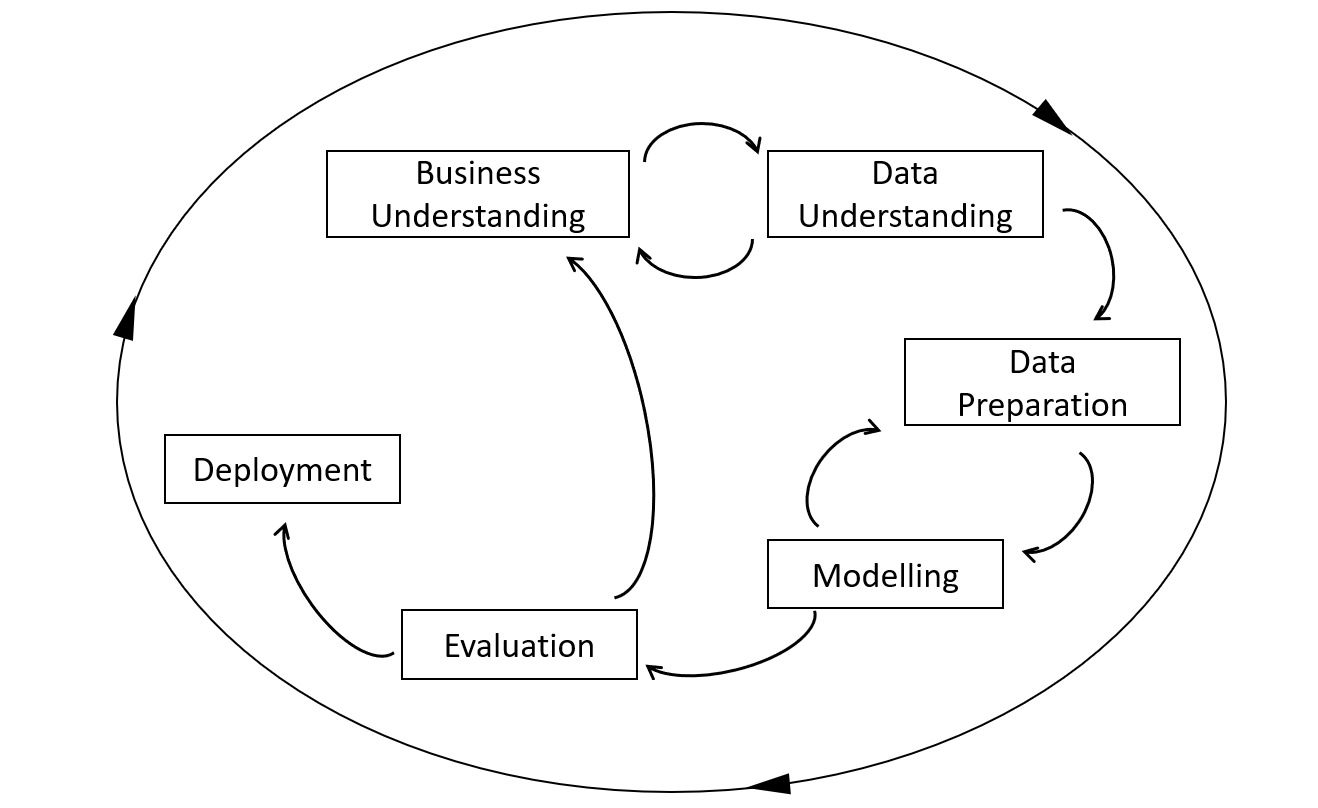
\includegraphics[width=\linewidth]{CRISP-DMGregor.png}
	\end{figure}
	Die Schritte Business Understanding und Data Understanding sind gleichzusetzen mit Kapitel 2 (Fragestellung) bzw. Kapitel 4 (Beschreibung Datensatz) Die eigentliche Entwicklung der Methode kann in die Schritte Data Preparation, Modelling, Evaluation und Deployment aufgeteilt werden. Die Schritte verschwimmen in der Praxis alle miteinander. Das eigentliche Konzept an dem sich orientiert wird besteht darin, dass das Modell schrittweise verbessert wird. Es wird also zuerst ein ‚einfaches‘ Modell entwickelt und dann nach einer Evaluation immer wieder verbessert, bis ein zufriedenstellendes Ergebnis vorliegt.
	
	\section{Daten}
	\subsection{Beschreibung Datensatz}	
	Je nach Methodenwahl werden unterschiedliche Daten benötigt. Wenn allerdings zusätzlich ein Neural Network trainiert werden soll ist es auch nötig einen bereits gelabelten Datensatz zum training zu haben.
	
	Zur Verfügung steht ein Datensatz mit 56005 Produkten in Form einer \texttt{.csv}-Datei. Bei den Produkten, die in den Daten erfasst wurden, handelt es sich um unterschiedliche Arten von Haushaltsgeräten. Die Produkte reichen dabei von Waschmaschinen und Wäschetrocknern bis zu Kühlschränken und Mikrowellen. Eine genaue Zusammenfassung welche Produkttypen in den Daten vorkommen, kann durch eine erste Datenbegutachtung nicht getroffen werden. Die Werte wurden aus den Produktseiten verschiedener eCommerce Seiten extrahiert. Die Aufteilung der Daten nach Quelle ist wie folgt:\\
	
	\begin{tabular}[h]{|l|r|}
		\hline 
		Quelle & Anzahl \\ \hline 
		shopee.my&24849\\
		appliancesconnection.us&21434\\
		sharafdg.ae&5443\\
		productreview.au&2502\\
		spencerstv.us&1777\\ \hline
	\end{tabular}
	\newline
	
	Nachdem die .csv Datei mithilfe von Pandas in ein Dataframe überführt wurde, erhält man die Nachfolgende Datenstruktur:\\
	
	\begin{tabular}[h]{|c|c|c|c|c|c|c|}
		\hline 
		id & source & name & productdescription & url & brand & modelnumber \\ \hline 
	\end{tabular}
	\newline
	
	Die Zeilen von Interesse sind ‚name‘ und ‚productdescription‘. In diesen Feldern stehen die Sequenzen, aus denen die Attribute extrahiert werden sollen. Außerdem ist der Datensatz bereits für die Attribute ‚brand‘ und ‚modelnumber‘ gelabelt. 
	(der Absatz könnte weggelassen werden. Um einen ersten Eindruck der Daten zu bekommen wird nachfolgen der erste Eintrag des Datensatzes aufgeführt:\\
	\begin{tabular}[h]{rp{11.2cm}}
		id & 000266f5e7ab2344315290174dfb75f7 \\
		source & appliancesconnection.us\\
		name & Broan TEN136WW\\
		productdecription & Broan TEN136WW Overview The Tenya 1 Series Under Cabinet Range Hood by Broan offers 2-speed motor with up to 250 CFM of ventilation. [...] Vertical/Horizontal Rectangular Duct 7 in. Vertical Round Duct 1 Year Limited Warranty\\
		url & https://www.appliancesconnection.com/broan-ten136ww.html?zipcode=20001\\
		brand & Broan\\
		modelnumber & TEN136WW
	\end{tabular}
	\newline
	\newline
	Bei der ersten Begutachtung der Daten sind einige Problemstellen und mögliche Störfaktoren:
	\begin{enumerate}
		\item “-Zeichen wird in der Zeile ‚productdescription‘ oft als Größen Bezeichnung benutzt: Dadurch denkt Pandas, dass der Satz/String vorbei ist und jedes weiter Komma wird als neue Zeile interpretiert
		\item Chinesiche Zeichen bei mind. einem Produkt
		\item Andere Sonderzeichen. Es gilt zu untersuchen ob diese verarbeitbar  oder Stör\-faktoren sind
		\item Verschiedene Quellen könnten zu verschiedenen Mustern führen. Es sollte beobachtet werden wie sich das Modell je nach Quelle verhält.
		\item Marke und Modellnummer sind bei mindestens einer Quelle sehr einfach zu bestimmen. Oft setzt sich der Produkttitel aus Marke und Modellnummer zusammen (siehe Beispieldatensatz). Hier sollte der Einfluss dieses Musters untersucht werden.
	\end{enumerate}

	\section{Methodenüberblick}
	Alle Methoden lassen sich unter dem Begriff Named Entity Recognition zusammenfassen.	Nachfolgend werden ausgewählte Methoden erklärt. Bei allen handelt es sich um Machine Learning Ansätze. 
	
	\subsection{Naive Bayes}
	Eine Möglichkeit des NER liegt darin das Klassifizierungsproblem mit einem Naive Bayes Klassifikators zu lösen. Bei Naive Bayes wird sich ‚supervised learning‘ zu nutzen gemacht. Es werden also gelabelte Trainingsdaten benötigt. Anhand der Trainingsdaten werden für alle Werte die Wahrscheinlichkeiten bestimmt, dass der Wert einer bestimmten Klasse zugehört (bzw. eine Hypothese erfüllt). In unserem Fall könnten die Werte die Wörter einer Sequenz und mögliche Klassen ‚Attribut‘, ‚Attributwert‘ und ‚Keins von beiden‘ sein. Nachdem die Wahrscheinlichkeiten bekannt sind, können anhand des Naive Bayes Klassifikators die ungelabelten Daten immer der Klasse mit der höchsten Wahrscheinlichkeit zugeordnet werden. Um eine erfolgreiche NER Methode auf Basis von Naive Bayes entwickeln zu können benötigt es noch weitere Schritte wie beispielsweise das Verlinken zwischen Attributen und Attributwerten.\\
	Der Naive Bayes Klassifikator ist ein weiteverbreitetes Mittel zur Textklassifizierung und wird beispielsweise bei Spam Filtern erfolgreich eingesetzt um Wörter in die Klassen ‚Spam‘ (Schlecht) oder ‚Ham‘ (Gut) einzuordnen. Allerdings ist der Ansatz wie bereits im Namen steht naiv. Er geht davon aus, dass keine Beziehungen zwischen den Werten bestehen. Diese sich also nicht gegenseitig beeinflussen. Diese Annahme ist kritisch bei der Textverarbeitung. In unserem Anwendungsfall könnte sich das unter anderem negativ auf die Extraktion von Attributwerten welche aus mehreren Wörtern zusammengesetzt sind auswirken. Bei solchen Attributwerten bestehen Abhängigkeiten zwischen mehreren Wörtern, die das Modell beachten sollte.
	\footnote{(Quelle: Text Mining for Product Attribute Extraction)
	(Quelle: https://course.elementsofai.com/de/3/3)}
	\subsection{CNNs}
	Neueste Ansätze verwenden CNNs zur Klassifikation. \cite{Zhu.2018} haben erfolgreich ein CNN verwendet um 2017 die genaueste Methode zur Named Entity Recognition von verschiedenen Biologieliteraturkorpora vorzustellen. Die GRAM-CNN genannte Methode hat laut den Autoren für das labeling von Biologieliteratur einen Genauigkeitsvorteil indem, nicht wie in klassischen LSTMs der ganze Satz betrachtet wurde, sondern nur die um ein Wort liegenden Nachbarworte. Die Worte, dieser N-Gram genannten Wortketten, werden in einem ersten Schritt zu einer Darstellung umgewandelt, die nicht das Wort selber enthält, sondern das Wort durch seine einzelnen Buchstaben als Vektor darstellt. Dazu wird dem Wort noch ein Part-of-Speech tag zugewiesen und der Character des Worts als Vektor dargestellt. 
	Die Vektorisierung erfolgt durch Abgleich der Worte mit vorgefertigte Bibliotheken die auf ähnlichen Korpora Vektoren berechnet haben. Das Part-of-Speech tag enthält Informationen zu Abhängigkeiten eines Wortes zu anderen. Eine Eingabe in das GRAM-CNN ist also ein n-gram, das wie beschrieben durch seine Buchstaben mit Zusatzinformationen dargestellt wird.
	Innerhalb des CNNs wird diese Information versteckt verarbeitet und es liefert die features der Worte an ein CRF in dem die Verbindung von mehreren Worten erkannt werden kann. Damit sind auch auseinander geschriebene zusammengehörige Worte als solche erkennbar.\\
	CNNs wurden auch in \cite{Lee.2019} und \cite{Lee.2020} verwendet um Produkteigenschaften aus Benutzerbewertungen zu extrahieren. Mit den extrahierten Eigenschaften werden von den Autoren letztlich Sentiment-Scores der Benutzerbewertungen erstellt, die nicht nur die Erwähnung von bewertbaren Wörtern zählen, sondern auch die relative Gewichtung von verschiedenen Eigenschaften des bewerteten Produkts herausfinden.\\
	\subsection{RNNs (LSTMs)}
	RNNs sind die Standardmethode für Textklassifikation, dabei wird meist die Spezialform der LSTMs verwendet.\footcite{Majumder.2018}
	RNNs verwenden wie die vorherigen Methoden Trainingsdaten um einen Klassifikator zu trainieren. Eingaben sind Texte aus denen bereits die Interessanten Textstellen mit ihrer Beschreibung extrahiert wurden. Damit wird ein Neuronales Netzwerk trainiert.
	Das trainierte Netzwerk ist dann in der Lage beliebige Texte einzulesen und die darin enthaltenen Entitäten in Form von Markennamen zu erkennen und zuzuordnen. Mit diesen Informationen sollte es möglich sein größere Korpora von Produktbeschreibungen automatisch mit Informationen anzureichern.

	\section{Implementierung}
	\subsection{Architektur} %Thilo
	Das gesamte Programm soll mithilfe von Python implementiert werden. Innerhalb von Jupyter Notebooks sollen Codeabschnitte einzeln ausführbar sein. Die weit verbreiteten Bibliotheken spacy und keras sollen als Grundbausteine verwendet werden, da sie nützliche Funktionen bereits implementieren.\\
	Spacy ist dabei zur Textbearbeitung und -vorbereitung nützlich. Darin enthalten sind Werkzuege zur Tokenisierung und speziellere Werkzeugen wie zum Stemming der Tokens. Damit könnten Wörter auf ihren Wortstamm zurückdekliniert werden.
	In Keras ist eine Verbindungsstelle zwischen python und der Tensorflow Bibliothek hergestellt. Tensorflow ist der für dieses Projekt notwendige Baustein um künstliche Neuronale Netzwerke einfach zu verwenden.
	
	Der Aufbau der Neuronalen Netze ist noch nicht endgültig festzulegen. Nach erster Implementierung werden verschiedene Tiefen und Zusammensetzungen von Ebenen ausprobiert um zu einem möglichst guten Ergebnis zu kommen. Dabei muss auch ein Ausgleich zwischen Geschwindigkeit und Genauigkeit der Klassifizierung gefunden werden.
	
	\subsection{Training/Validation/Testing der ML Methode} %Thilo
	Der Datensatz soll in drei Teile aufgespalten werden. Diese drei Teile werden zum Training, der Validierung und für die abschließenden Tests verwendet. 
	
	Das Trainingsset soll der größte Teil mit etwa 70\% der Daten sein. Mit diesen Daten soll das Netzwerk mit seinen Gewichten darauf trainiert werden Markennamen und Produktnummern zu erkennen.
	Je 15\% sollen für Validierung und Testen verwendet werden.
	Die Validierung ist zur Feinjustierung von Hyperparametern zuständig.
	Das Testen soll vor allem overfitting des Modells überprüfen. Wenn ein auf den Trainingsdaten gut funktionierendes Modell trainiert wurde sollte es ähnlich gut für die bisher ungesehenen Testdaten funktionieren. Ist dies nicht der Fall, könnte ein Vergleich auf Overfitting hindeuten.
	
	Abschließend sollen verschiedene automatisch mitgeschnittene Metriken in Grafiken aufbereitet werden um die Ergebnisse anschaulich darstellen zu können.
		
	\subsection{Verbesserungsmöglichkeiten/Mögliche Erweiterungen} %Gregor
	Mit dem derzeitigen Plan ein LSTM zu verwenden sind folgende Verbesserungs\-möglichkeiten vorgesehen.
	
	\subsubsection{CRF}
	Eine Möglichkeit besteht darin Conditional Random Fields (CRF) wie in \cite{Majumder.2018} und \cite{Zheng.2018} zu verwenden. Dabei würde CRF die Aufgabe der Output Schicht übernehmen und wäre für das Labeling zuständig. Wird keine CRF-Schicht verwendet, dann berechnet das LSTM das passende Label für jedes Token eigenständig und unabhängig. Durch die CRF-Schicht passiert das Labeling der gesamten Eingabesequenz auf einmal, wodurch es möglich ist, die Abhängigkeiten zwischen Wörtern, die in Nachbarschaft zueinander stehen, zu berücksichtigen. CRFs sind immer dann hilfreich, wenn Attributwerte gesucht werden, die sich aus mehreren Wörtern zusammensetzen können. In diesem Projekt ist das das Attribut ‚Marke‘ bzw. ‚brand‘. Markennamen bestehen nicht selten aus mehr als einem Wort (Beispiele aus dem Datensatz: ‚Fulgor Milano‘, ‚Fisher Paykel‘, ‚Ready Hot‘, …). CRF hilft dabei, auch diese Markennamen als einen Attributwert, der aus mehreren Tokens besteht, zu erkennen. 
	
	\subsubsection{Attention}
	Eine weitere Verbesserung könnte durch eine Attention Schicht wie in \cite{Majumder.2018} und \cite{Zheng.2018} zustande kommen. Diese würde nach den LSTM Schichten und vor der Output Schicht eingefügt werden. Attention wird bei NER dafür eingesetzt, um den Fokus auf die wichtigen Konzepte in den Sequenzen zu legen, anstatt alle Informationen gleich zu behandeln. Dadurch wird das CRF bzw. die Output Schicht bei der Entscheidung optimal unterstützt und kann sich auf diese Konzepte fokussieren. Bei Attention wird für jedes Token ein Wert lt berechnet, der beschreiben soll, wie viel Beachtung einem Token geschenkt werden soll, um den Kontext der Nachbarn zu beschreiben. 
	Allerdings legen die Dokumente nah, dass durch Attention nicht unbedingt verbesserte Labeling Ergebnisse erzielt werden können. Die Schicht wird dort eher dazu verwendet, die Entscheidungsfindung des Netzwerks anhand der als wichtig erkannten Tokens zu beschreiben und nachvollziehen zu können. 
	
	
	\printbibliography[title=Literaturverzeichnis]
\end{document}
